\documentclass[supercite]{Experimental_Report}
\usepackage{ctex}
\title{~~~~~~新生实践课~~~~~~}
\author{周子闰}
\school{计算机科学与技术学院}
\classnum{CS2404}
\stunum{U202414650}
\instructor{陈加忠} % 该系列实验报告模板由华科大计院教师陈加忠制作
\date{2024年11月24日}
\usepackage{indentfirst}
\usepackage{verbatim}
\usepackage{algorithm, multirow}
\usepackage{algpseudocode}
\usepackage{amsmath}
\usepackage{amsthm}
\usepackage{framed}
\usepackage{mathtools}
\usepackage{subcaption}
\usepackage{xltxtra} %提供了针对XeTeX的改进并且加入了XeTeX的LOGO, 自动调用xunicode宏包(提供Unicode字符宏)
\usepackage{bm}
\usepackage{tikz}
\usepackage{tikzscale}
\usepackage{pgfplots}
%\usepackage{enumerate}

\pgfplotsset{compat=1.16}

\newcommand{\cfig}[3]{
  \begin{figure}[htb]
    \centering
    \includegraphics[width=#2\textwidth]{images/#1.tikz}
    \caption{#3}
    \label{fig:#1}
  \end{figure}
}

\newcommand{\sfig}[3]{
  \begin{subfigure}[b]{#2\textwidth}
    \includegraphics[width=\textwidth]{images/#1.tikz}
    \caption{#3}
    \label{fig:#1}
  \end{subfigure}
}

\newcommand{\xfig}[3]{
  \begin{figure}[htb]
    \centering
    #3
    \caption{#2}
    \label{fig:#1}
  \end{figure}
}

\newcommand{\rfig}[1]{\autoref{fig:#1}}
\newcommand{\ralg}[1]{\autoref{alg:#1}}
\newcommand{\rthm}[1]{\autoref{thm:#1}}
\newcommand{\rlem}[1]{\autoref{lem:#1}}
\newcommand{\reqn}[1]{\autoref{eqn:#1}}
\newcommand{\rtbl}[1]{\autoref{tbl:#1}}

\algnewcommand\Null{\textsc{null }}
\algnewcommand\algorithmicinput{\textbf{Input:}}
\algnewcommand\Input{\item[\algorithmicinput]}
\algnewcommand\algorithmicoutput{\textbf{Output:}}
\algnewcommand\Output{\item[\algorithmicoutput]}
\algnewcommand\algorithmicbreak{\textbf{break}}
\algnewcommand\Break{\algorithmicbreak}
\algnewcommand\algorithmiccontinue{\textbf{continue}}
\algnewcommand\Continue{\algorithmiccontinue}
\algnewcommand{\LeftCom}[1]{\State $\triangleright$ #1}

\newtheorem{thm}{定理}[section]
\newtheorem{lem}{引理}[section]

\colorlet{shadecolor}{black!15}

\theoremstyle{definition}
\newtheorem{alg}{算法}[section]

\def\thmautorefname~#1\null{定理~#1~\null}
\def\lemautorefname~#1\null{引理~#1~\null}
\def\algautorefname~#1\null{算法~#1~\null}
\setlength{\parindent}{2em}
\begin{document}

\maketitle

\clearpage

\pagenumbering{Roman}

\tableofcontents[level=2]

\clearpage

\pagenumbering{arabic}

\section{网页整体框架}
日常使用的网页逻辑非常自然,通过一级一级的导航进入到自己想要的网页。导航栏这一个实用的工具深受人们认可,我也利用我的储备试图制作了一个这样的导航栏。\\  当然,这个导航栏相当简陋,由于我没有使用CSS,每次修改样式都需要一次一次改,这很不利于后期的维护。但是能秉承着跑起来的bug就不去动它的理念,我还是在我的网页中使用了这个简陋的导航栏,它使得用户可以在所有不同的页面中切换,当然也就实现了从一到多从多到一的切换。\\  下面这个思维导图反应了这个网页的逻辑关系,而不是操作关系--因为任何一个页面都可以切换到其他的页面,而不是简单的一对多。

\begin{figure}[h]
	\begin{center}
		\includegraphics[scale=1.0]{images/MINDMAP.png}
		\caption{网页逻辑图}
		\label{fig1-1}
	\end{center}
\end{figure}

\newpage

\section{主页设计}

主页由导航栏,标题,正文组成。

\begin{figure}[htb]
	\begin{center}
		\includegraphics[scale=0.05]{images/index.png}
		\caption{主页举例}
		\label{fig2-1}
	\end{center}
\end{figure}

其中导航栏部分代码分为五个部分,分别为nav选择器,nav ul选择器,nav ul li选择器,nav ul li a选择器和nav ul li:a:hover选择器。\\  其中nav选择器设置了导航栏的宽度,颜色(深灰色),文导航栏文本内容为白色,并将导航栏固定在页面的视口中不随滚动条滚动,并且用top:0和left:0将导航栏定位在视口的顶部和左侧,height设置为100\%使其高度占满整个视口,将padding-top和padding-bottom分别设置为20px以添加20像素的页边距,最后使用border-radius来给导航栏四个角添加圆角。而nal ul选择器则实现了移除默认的列表项目标记,内边距和外边距。nav ul li选择器则为每个列表项设置了上下20像素的外边距和左右0像素的外边距。nav ul li a选择器设置了链接的一些显示效果,把连接文本颜色显示为白色,字体大小为18像素(更饱满),链接显示为块级元素使其占满列表项的宽度,并设置了背景颜色变化的过渡效果为0.3s。最后,nav ul li a:hover使得鼠标悬停时把背景颜色改为稍浅的灰色(\#555)。\\  总之,这个导航栏最后的效果还是让我挺满意的。
\begin{figure}[h]
	\begin{center}
		\includegraphics[scale=0.15]{images/maindex.png}
		\caption{部分代码展示}
		\label{fig2-2}
	\end{center}
\end{figure}
对于body选择器和主内容区字体页边距的大小有许多同理之处,对这一内容不再赘述。在body选择器中我用background-image来设置了一张页面背景图,并且将尺寸设置为cover以覆盖整个页面,并且将display设置为flex来使子元素可以灵活排列。而在主内容区,我将左页边距设置为270像素,前面已经说明导航栏宽度为250px,这里多留一点点空间,然后width:calc(100\%-270px)使得页面填满整个画面而不留空白.背景色调为半透明的白色,不透明度调高是不希望背景图片喧宾夺主。
\\  这里页脚的页面设计和主内容区一致,但是最后出于一些考虑我删除了页脚部分的内容,使得这一部分没有在网页中展示。
\begin{figure}[h]
	\begin{center}
		\includegraphics[scale=0.25]{images/XYSSJ.png}
		\caption{响应式设计代码展示}
		\label{fig2-3}
	\end{center}
\end{figure}
最后通过一个简单的响应式设计,使得当用手机等小屏幕设备打开网页时调整网页的布局使得能够适应屏幕大小。网页不适应小屏幕设备是我日常使用网页时的一个痛点,因此我对这个适配做了一点点努力。
\\注:标题和末尾“如对本网页的内容有任何异议,可到681寝室找本人进行修改,本人竭力保证内容让您满意。”是本人为了实现网页内容“细思极恐”的效果而写,不是语病,而是在文本内容上标新的一点小尝试。
\newpage

\section{分页面设计}
	\subsection{音乐}
	
	\begin{figure}[h]
		\begin{center}
			\includegraphics[scale=0.05]{images/music1.png}
			\caption{音乐-1}
			\label{fig3-1}
		\end{center}
	\end{figure}
	
	页头下简单的标题和简介之后,我放上了我的QQ音乐的截图,展示了我的一些歌单,初步传递了我的音乐志趣。
	
	\begin{figure}[h]
		\begin{center}
			\includegraphics[scale=0.05]{images/music2.png}
			\caption{音乐-2}
			\label{fig3-2}
		\end{center}
	\end{figure}
	
	而在主内容区,我分两栏展示我喜欢的一些音乐类型、歌手和个别单曲。每个板块包括一张图片(在个别其他的网页中,图片可能不只一张)(出于硬盘占用考虑,我只放一张,但是我其实想放更多...)和一些简单的评论和感想。下面展示一些代码,说明我的分页设计思路:
	
	\begin{verbatim}
		设置大图样式 (large-image):
		text-align: center;  /* 将大图居中对齐 */
		margin-top: 20px;  /* 设置大图上方的外边距 */
		
		.large-image img:
		width: 100\%;  /* 图片宽度自适应100\% */
		max-width: 800px;  /* 图片最大宽度为800px */
		height: auto;  /* 图片高度自动调整以保持比例 */
		border-radius: 10px;  /* 图片四角圆滑 */
		
		设置音乐展示的样式 (music-gallery):
		display: grid;  /* 使用网格布局显示音乐项目 */
		grid-template-columns: repeat(2, 1fr);  /* 每行显示2个项目 */
		gap: 20px;  /* 网格项目之间的间距为20px */
		margin-top: 20px;  /* 顶部间距为20px */
		
		设置每个音乐项的样式 (music-item):
		text-align: center;  /* 音乐项文本居中对齐 */
		background-color: rgba(0, 0, 0, 0.05);  /* 设置背景颜色为浅灰色 */
		border-radius: 10px;
		padding: 15px;
		box-shadow: 0 4px 8px rgba(0, 0, 0, 0.1);  /* 设置阴影效果 */
		transition: transform 0.3s, box-shadow 0.3s;  /* 为变换和阴影添加过渡效果 */
		
		.music-item:hover:
		transform: translateY(-5px);  /* 悬停时音乐项向上移动5px */
		box-shadow: 0 8px 16px rgba(0, 0, 0, 0.2);  /* 悬停时加大阴影效果 */
		
		.music-item img:
		width: 100\%;
		max-width: 200px;
		height: auto;
		border-radius: 8px;
		margin-bottom: 10px;
		
		.music-item h3:
		margin: 10px 0 5px;
		font-size: 20px;
		
		.music-item p:
		font-size: 14px;
		color: \#555;  /* 将 #555 转义为 \#555 */
		
	\end{verbatim}
	
	总体来说,使用网格布局实现分栏展示音乐内容,用:hover伪类实现悬停时的上浮效果。老实说,实现这一步时,我的内心欢呼雀跃,因为这是一个我真的能在各种网站中见到的交互形式,流畅的悬浮看起来赏心悦目,而我居然实现了!我非常自豪。
	
\subsection{游戏}

\begin{figure}[h]
	\begin{center}
		\includegraphics[scale=0.05]{images/games.png}
		\caption{游戏}
		\label{fig3-3}
	\end{center}
\end{figure}
框架大同小异,不作赘述。展示我不多的Steam库存,贴上了我喜欢的游戏海报或者截图,介绍了一下我喜欢玩的一些游戏,本想添加Minecraft的内容,但是因为文件快超大小了,只好作罢。
\subsection{魔方}
\begin{figure}[h]
	\begin{center}
		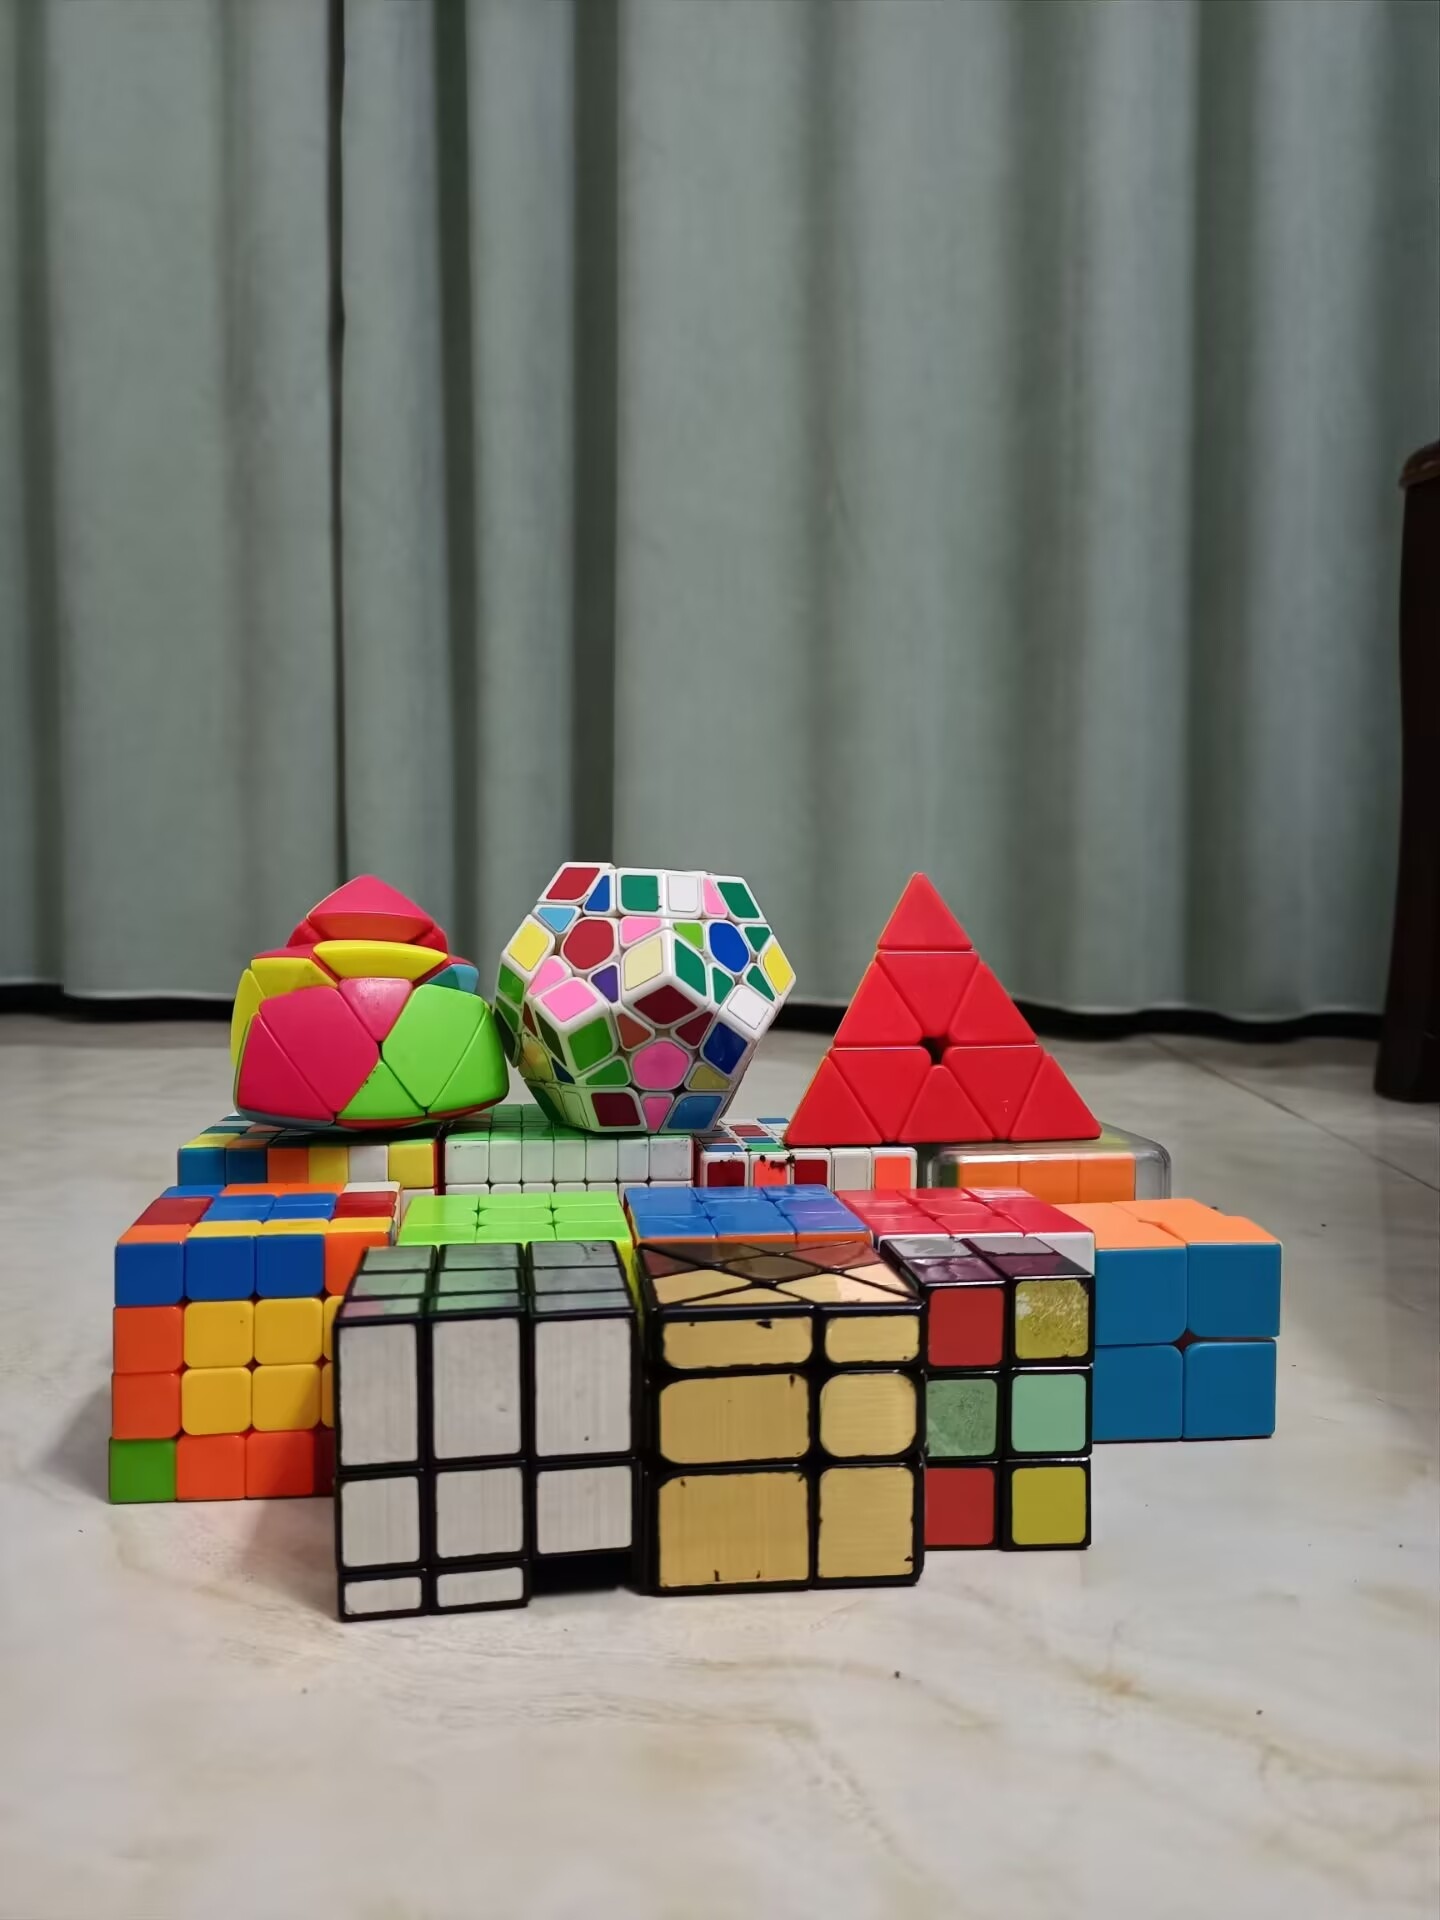
\includegraphics[scale=0.05]{images/cube.png}
		\caption{魔方}
		\label{fig3-4}
	\end{center}
\end{figure}
展示了我玩过的魔方和一次打破个人记录的计时器截图,写了一些玩了这么久魔方的感想。它承载我很多很多回忆,度过了很多时光,交到了一些朋友。
\newpage
\subsection{书法}
\begin{figure}[h]
	\begin{center}
		\includegraphics[scale=0.05]{images/calligraphy.png}
		\caption{书法}
		\label{fig3-5}
	\end{center}
\end{figure}
展示了我这么久以来写过的古帖的一部分,初二开始练字,高一下册开始写古帖,由于没有老师教纯粹自己摸索,进步有些慢而且状态有起伏。如今也算小有成色,在同龄人面前堪堪拿得出手,让我有了继续走下去的动力。\\注:由于文件大小的限制,没能展示我为练字添置的笔具。
\subsection{电影}

\begin{figure}[h]
	\begin{center}
		\includegraphics[scale=0.05]{images/movies.png}
		\caption{电影}
		\label{fig3-6}
	\end{center}
\end{figure}
贴点喜欢的电影。电影真是一种伟大的艺术,人们居然能用自己的眼睛去经历故事。

\newpage

\section{网页设计小结}
网页设计对我来说是一项很有挑战性的任务,最初对我来说,最难的是想象出自己想要的网页画面。刚开始我并不知道我想要一个什么样的网页,东写一点西写一点,没有规划性。但是当我想到导航栏时,我觉得先做一个导航栏会是一个很好的想法——我可以一边做这个导航栏,一边想我的个人主页需要做些什么内容,然后把它们填进导航栏里,而且就算我后面有新的想法,也可以很方便地添加。于是我上网查找导航栏的制作方法,一步一步地调节它的样式使得它符合我对于导航栏的期待——圆角,悬浮特效,字体,当然在这过程中我也解决了一些我刚开始没有想到的方面,比如调节合适的页边距等等。最后这个导航栏完工的时候,我非常满意,因为它完全符合我对一个导航栏的想象,实现了我期望的功能。
然后我开始着手设计网页的主体部分,刚开始主内容区我把宽度设计为视窗的100\%,这导致了糟糕的后果——有一部分主页面被不透明的导航栏遮盖住了,我尝试使导航栏透明化以减少遮挡,但是效果仍然不理想,因为导航栏和主内容区的内容重叠了,非常影响阅读。最后查找了相关的资料我把width设置为100\%-270px,这样主页面就会和导航栏分开,并且中间留出了一点点空间,使得整个页面不至于太拥挤。\\然后我按照教程结合自己的想象写了页头和页脚,但是在后来的分栏设计中加入页脚会使页脚单独分掉一半的页面,这很丑陋,于是我删去了页脚。然后我便开始往主内容区中加入内容。
当index网页做完之后我仿照这个模式制作了其他网页。然后在普通地插入图片并且介绍了一个音乐类型之后我发现这样的表现形式过于单调,而且排版也会因为文字长度地不同而显得并不整齐。这时我想到了购物软件上的商品呈现方式:一块一块地切分区域,在每一个区域中加入图片和相应的文字说明,并且当光标移动到相应的区域的时候会出现交互。于是我继续上网学习如何分栏展示,如何设置上浮效果。幸运的是这些内容都有详细的介绍和教程,我仿照这些教程做出了音乐展示的模块,并且按照我的想象调节了字体等内容,总体来说效果还算令人满意,接下来我就以这个为模板做完了其他的网页的框架,然后我就开始向其中填充我的内容。最终因为文件大小的限制,我忍痛删除了一些内容,并且没有使用更复杂的动画。
当我打开这个网页时,我的内心充满了满足感。虽然它仍然非常简陋,也没有涵盖我想要的所有效果和内容,但是它也不至于粗制滥造,它实现了我想要的很多效果,而且它的板块有了我很喜欢的圆角和上浮效果,并且可以后期升级维护。\\总之,通过这次网页设计,我进一步学习了html语言。这个语言在实现页面效果时有点类似LaTex,你可以很方便的用语言告诉计算机你需要实现什么样的效果,可以很方便地指定一些特定的参数,虽然这些参数的使用需要一些实践的经验。而DW实时可视化的功能可以让我更快捷方便地查看我编辑的效果,可以看出我使用的参数的效果,这点比一些LaTex编译器要更“新手友好”一些。\\当然我的能力还十分有限,我曾想做一个效果,在鼠标点击上浮的展示模块中时可以跳出一个更大的窗口覆盖掉这个网页,这个网页的底部有更多相关的图片,当鼠标在图片上方停留时会放大展示图片,但是最后由于太复杂且增加的图片会大大增加内存占用,我放弃了推进这个功能。或许未来我继续学习,可以实现我想要的这一效果。
\newpage

\section{课程的收获和建议}

对于学习这门课程来说,最重要的是实践,但是实践所需要的基本知识又非常重要。所以提前预习,上课认真听讲可以更早更牢固地掌握基本的知识,实践时可以更投入地去运用知识解决问题。

\subsection{计算机基础知识}

我5岁就捣鼓过计算机了,买电脑时计算机的组成部分也了解得差不多了。这一部分对我来说意义不大。

\subsection{文档撰写工具LaTeX}
挺新奇的一个工具,刚开始非常不适应,因为用习惯了word的可视化编辑。但是用word的逻辑就是眼见即所得,对于一些细微的调整(比如图片的位置调整)有时会引起排版乱序的效果,但是LaTex就不会出现这个问题,在LaTex里你说啥就是啥,就是不能可视化,如果有调整就不是很方便。我觉得课程中最让我不适应的地方是没有一个很舒服的逻辑过渡时期,要让习惯了word甚至连word都不会用的人理解LaTex的逻辑,可以在最开始时加一点小小的实践题,让同学们先感受一下如何对文档效果颐指气使。
\subsection{编程工具Python}
Py很强,但是课程的矛盾也很明显,短短时间内就要讲明白基础又要学以致用,这是很难实现的。既然课程的目的是实践,而同学们又学正在学C,不如大篇幅地介绍两者的逻辑相似之处和不同之处,然后在实践作业设计梯度更为平滑但是量稍多一些的题目引导同学们在实践中去查阅、学习这门编程语言,而不是把它当作独立于C的一个编程语言从头开始讲。
\subsection{图像设计软件Photoshop}
之前没怎么接触过这类型的软件,感觉只是基本了解了这个软件和图片处理类型的基本操作,我在网上看到过一些PS大神的操作,感觉他们对于这个软件、对于图片的理解非常深刻,我还需要继续学习。对于教学,可以适当提供一些拓展阅读材料,不必要求过高,但是可以给同学更多的接触、运用、实践机会。
\subsection{版本管理软件Git}
通过课程学习,我学会了使用git的一些基本流程,虽然对命令行的运用还很生疏,但是相信随着日后的开发经验的丰富一定会越来越熟练。By the way,或许在课堂上也可以介绍一些其他的Git工具,如tortoisegit,相比git拥有可视化操作并且有更直观的分支管理视图,更容易上手,可以让同学们了解一下。
\subsection{网页制作Dreamweaver}
DW这种既可视化又能颐指气使地指定效果的编程体验太好了,感觉像是Word+LaTex一样。这个课堂让我第一次接触到了前端的开发,并且通过自己的努力取得了自己还算满意的成果。感觉没啥可以建议的了,主要是实践出真知,真的是实践中才感受到开发的美的魅力,虽然我还算不上实际开发哈哈哈。
\end{document}
%\nocite{*} %% 作用是不对文献进行引用,但可以生成文献列表

%\bibliographystyle{Experimental_Report}
%\bibliography{Experimental_Report}
%\setcounter{secnumdepth}{0}
%\appendix

%\section{附录A 功能模块一实现的主要源程序}

%\noindent


